% ［架空の記入例・提出不可］通常ビルドには読み込まれません．
% 必要な構造だけをchapters/04-method.texへ移し，架空内容を置換してください．
\chapter{提案手法}

\begin{center}
  \UsamiFictionalExampleNotice
\end{center}

\section{全体構成}
本研究では，少数症例下の腹部CT多臓器領域分割を対象に，条件付き潜在拡散モデルで画像と臓器ラベルの対応を保った合成対を生成する．3D U-Net\cite{cicek20163dunet}を分割器とし，潜在空間での生成にはRombachら\cite{rombach2022ldm}の考え方を用いる．処理全体を図\ref{fig:method-overview}に示す．

\begin{figure}[tb]
  \centering
  % SVG原稿とPDF版をexamples/figures/へ同梱している．
  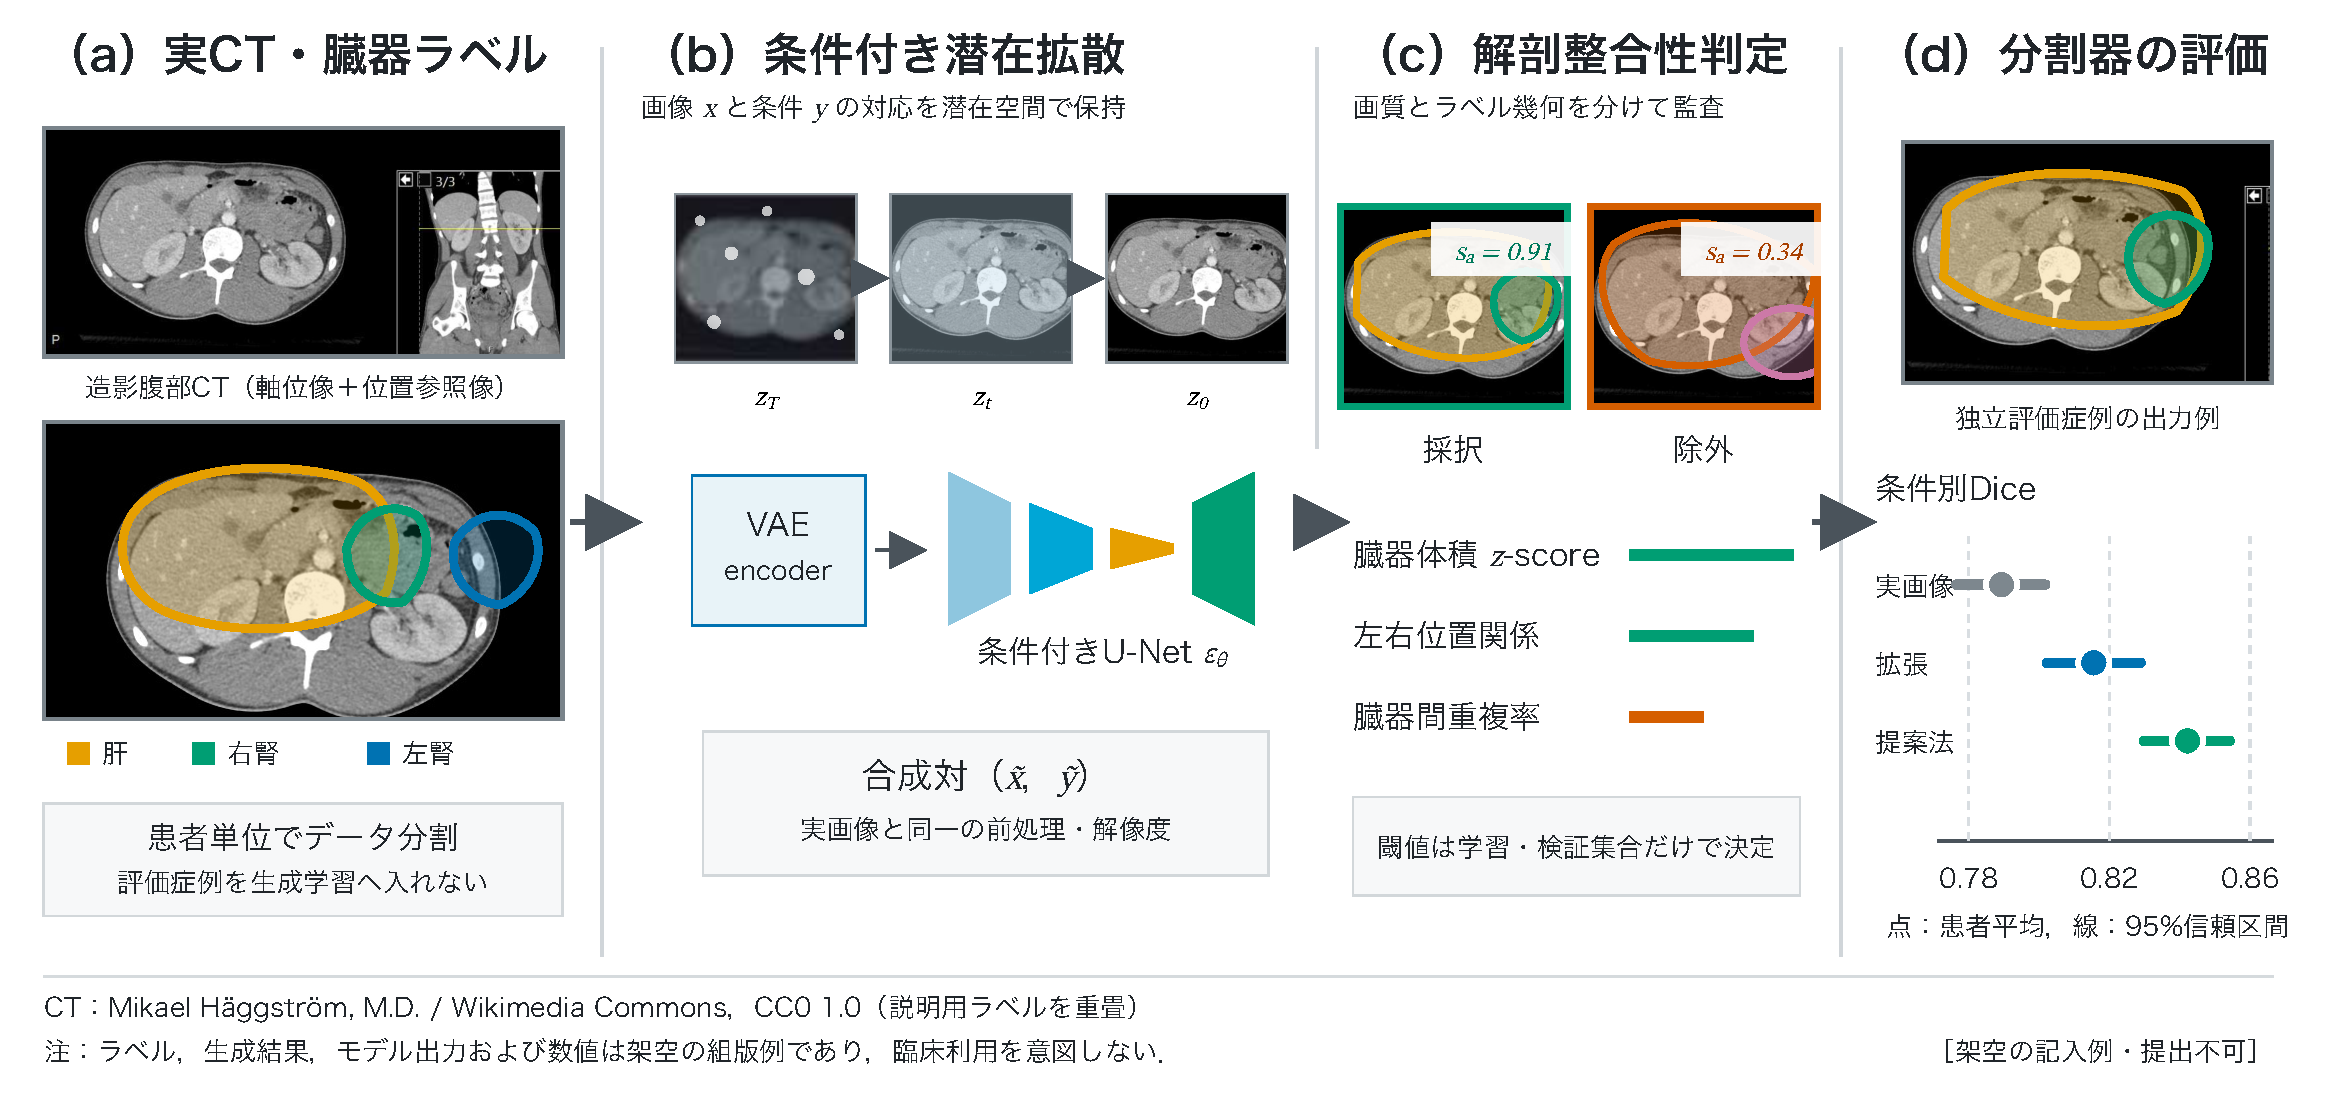
\includegraphics[width=\textwidth]{examples/figures/ct-diffusion-pipeline.pdf}
  % 図題は図本体より下へ置く．
  \caption{解剖構造保持拡散データ拡張の処理フロー}
  \label{fig:method-overview}
\end{figure}

図\ref{fig:method-overview}の解剖整合性判定では，臓器体積，左右臓器の位置関係，臓器間重複率を検査する．閾値は学習集合と検証集合だけから決定し，評価集合に合わせて変更しない．これにより，生成画像の視覚的な自然さと，条件ラベルの幾何学的妥当性を分けて評価する．

\section{学習目的関数}
患者$i$のCT体積を$x_i$，臓器ラベルを$y_i$，分割器の出力を$f_\theta(x_i)$とする．実画像と採択済み合成画像を同じミニバッチへ入れ，次の目的関数を最小化する．

\begin{equation}
  \mathcal{L}(\theta)
  =\mathcal{L}_{\mathrm{Dice}}
  +\lambda_{\mathrm{ce}}\mathcal{L}_{\mathrm{CE}}
  +\lambda_{\mathrm{ana}}\mathcal{L}_{\mathrm{ana}}.
  \label{eq:segmentation-objective}
\end{equation}

式\eqref{eq:segmentation-objective}の第1項と第2項は領域重複とボクセル分類を評価し，第3項は隣接すべき臓器の過度な離隔および重複を罰する架空の正則化項である．各係数は患者単位の検証集合で選択する．

\section{実装条件}
CT値を架空の範囲$[-150,250]$ HUへ切り詰め，$[0,1]$へ線形正規化する．分割器への入力は$96\times96\times96$ボクセルのパッチとし，AdamW，初期学習率$10^{-4}$，最大500 epochで学習する．検証Diceが50 epoch改善しない場合に停止し，全条件で更新回数を揃える．
